\documentclass{sigkddExp}

\begin{document}
%
% --- Author Metadata here --- -- Can be completely blank or contain 'commented'
% information like this... \conferenceinfo{WOODSTOCK}{'97 El Paso, Texas USA} %
% If you happen to know the conference location etc. \CopyrightYear{2001} %
% Allows a non-default  copyright year  to be 'entered' - IF NEED BE.
% \crdata{0-12345-67-8/90/01}  % Allows non-default copyright data to be
% 'entered' - IF NEED BE. --- End of author Metadata ---

\title{Patched-FLANNEL: COVID-19 X-ray Image Classification}
\subtitle{\url{https://mediaspace.illinois.edu/media/t/1_atvzrp1d}}

\numberofauthors{4}

\author{\alignauthor Maneesh Kumar Singh\\
    \affaddr{University of Illinois at Urbana-Champaign}\\
    \email{mksingh4@illinois.edu}
    \alignauthor Raman Walwyn-Venugopal\\
    \affaddr{University of Illinois at Urbana-Champaign}\\
    \email{rsw2@illinois.edu}
    \alignauthor Satish Reddy Asi\\
    \affaddr{University of Illinois at Urbana-Champaign}\\
    \email{sasi2@illinois.edu}
    \alignauthor Srikanth Bharadwaz Samudrala\\
    \affaddr{University of Illinois at Urbana-Champaign}\\
    \email{sbs7@illinois.edu}
}

\date{28 March 2021}
\maketitle
\begin{abstract}
    \textbf{Objective:}
    Detecting COVID-19 using Chest X-Ray (CXR) images is becoming increasingly
    popular in deep learning research. When training deep neural networks, large
    and balanced datasets are preferred. However, since COVID-19 is new, there
    are a limited number of CXR images available which results in a challenge
    for training deep neural networks. Existing research has shown different
    approaches to address this imbalanced data issue. Two notable studies are
    FLANNEL (Focal Loss bAsed Neural Network EnsembLe) model and a patch-based
    classifier that works on segmented versions of the lung contours. We
    propose merging these two concepts together to improve performance of
    detecting COVID-19 in CXR images.

    \textbf{Materials and Methods:}
    As a pre-processing step, use a segmentation network to create a masked CXR
    images that only displays the lung areas. Replace base models in FLANNEL
    with patch-based classifiers that take masked image as input. The
    patch-based classifiers are used for the ensemble.

    \textbf{Results:}
    We are able to reproduce FLANNEL with updated datasets. We created a
    segmentation network that can produce masks of the lung contours for CXR
    images and successfully used it to generate masked  CXR images of the
    updated FLANNEL datasets.The FLANNEL base models were successfully updated
    to be patch-based classifiers. The overall modifications resulted in similar
    performance of the original FLANNEL architecture, where some metrics
    improved while others decreased.


    \textbf{Discussion:}
    We saw improvement in metrics when training the base models and FLANNEL
    ensemble over updated dataset. Since no parameters were changed, we
    suspect that this is due to the large increase of COVID-19 images in the
    dataset compared to when the FLANNEL paper was written. When training
    the patch-based models, we noticed that some patch-based models slightly
    improved in performance while others slightly decreased but there were no
    major differences.

    \textbf{Conclusion:}
    With the Patched FLANNEL barely outperforming FLANNEL in certain metrics, we
    believe there is merit to conduct further research to determine if more
    improvements can be made. Potential areas that can be further developed are
    but not limited to; segmentation, data augmentation, changing number of
    patches, changing size of patch and more. However, it should be noted that
    the largest improvement in overall metrics when compared to the original
    FLANNEL with the old dataset is due to the updated dataset having a large
    increase in COVID-19 images. This highlights how crucial getting quality
    data is to improve performance on models.

\end{abstract}

\section{Introduction}
Coronavirus disease 2019 (COVID-19) is a contagious disease caused by severe
acute respiratory syndrome Coronavirus 2 (SARS-CoV-2). It has spread worldwide
leading to an ongoing pandemic. This pandemic has ravaged the world on an
unprecedented scale. By April 2021, 141 million people have been infected and
there are over 3 million deaths \cite{whocovid1920-apr-21}. Chest X-Ray (CXR) is
one of the important, non-invasive clinical diagnosis tools that helps to detect
COVID-19 and other pneumonia for affected patients.

Using deep learning for X-ray classification is an ongoing research area and
recently there have been promising models proposed for COVID-19 classification.
The problem that all of these models face is an imbalanced dataset due to the
limited number of COVID CXR images available.

FLANNEL is a COVID-19 CXR classification model proposed by Zhi Qiao et al.
\cite{10.1093/jamia/ocaa280} that has been shown to accurately detect COVID-19
even when trained with only 100 available COVID-19 x-ray images. There are two
core components for the FLANNEL architecture, the first is that it uses an
ensemble \cite{58871} of five independent base models that predict the
classification of the CXR. Each of the predictions are then passed through
another neural weight network to determine the final prediction classification.
The goal of the ensemble is to increase the robustness and accuracy of the
network since each base model should capture patterns in the images
independently \cite{combine}. The second core component for the FLANNEL is its
use of the special Focal Loss \cite{lin2018focal} function, a modification of
the standard cross-entropy loss that places a focus on the imbalance negatives
by applying down-weights to well-classified examples. Focal Loss has been known
to improve performance for imbalanced datasets.

Park et al. \cite{pmid32396075} has also created a deep learning model that has
been proven to be effective on detecting COVID-19 when trained with limited
datasets. The approach taken was to first detect lung contours of the CXR and
perform segmentation. The motivation for performing segmentation first is that
the patch based model focuses on the lung area since it’s the primary region of
interest used to perform analysis.  In general, standard biomarkers
\cite{pmid32396075} from CXR images analyzed are the following
\begin{enumerate}
    \item Lung Morphology
    \item Mean Lung Intensity
    \item Standard Deviation of Lung Intensity
    \item Cardiothoracic Ratio (CTR)
\end{enumerate}


Thus it could be observed that most of the initial diagnosis is carried out from
CXR images by concentrating on the lung area. We find this strategy also
makes the model less susceptible to noise happening outside the lung region.
After the lungs have been segmented, patch-based classification is performed.
Patch-based classification involves selecting random crops or patches across the
image for a set number of times and then performing classification on each
patch. Afterwards, the final prediction of the image is made by majority voting
based on the prediction of each patch. The advantage of using a patch-based
approach for classification is that since the classification is on a smaller
part of the image, the network has a higher chance of recognizing “local”
patterns, unfortunately the disadvantage of using a patch-based approach is more
likely for the image to not recognize “global” patterns throughout the whole
image. Based on the conclusion provided in the patch based paper
\cite{pmid32396075} by Park et al., it is clear that the patch-based
classification outperformed the models that used the whole image for a limited
train set data. As we have an imbalanced dataset with limited COVID-19 CXR
images, we were optimistic that utilizing patch-based classification models for
the FLANNEL ensemble with the combination of focal loss optimization would
result in a performance improvement.

Our goal was to take the novel ideas of each approach listed above with the goal
of improving performance. To accomplish this we made modifications to the
existing FLANNEL architecture by first pre-processing the CXR images by
performing segmentation of the lung contours. Afterwards, we updated the
independent base models in the ensemble to be patch-based classifiers. We call
this new architecture \textbf{Patched FLANNEL}. The network structure is shown in
Figure \ref{fig:improve} and similar to FLANNEL consists of two-stage approach.

\begin{figure*}[h]
    \centering
    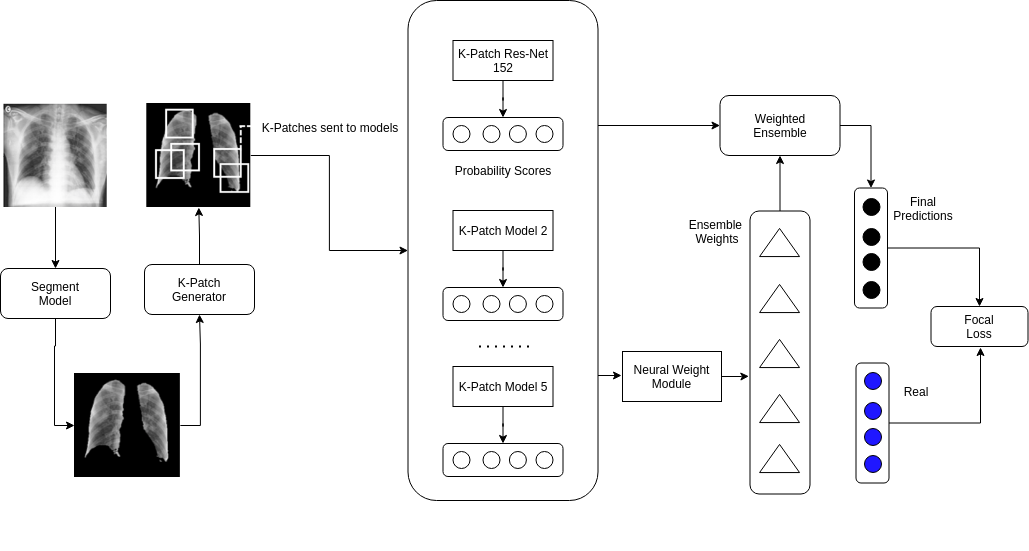
\includegraphics[width=0.8\textwidth]{../doc/images/Flannel_Improved_Latest.png}
    \caption{FLANNEL Improvement}
    \label{fig:improve}
\end{figure*}

\subsection{Related Work}

Here we discuss some of the related works that are being carried out in this
area on using deep learning techniques to detect COVID-19. Most of these works
either used CXR or CT scans for patients to detect COVID-19. Our current
research also falls in the same lines to accurately classify the patients CXR
images to COVID-19 class or non COVID-19 classes.

\subsubsection{AI-COVID}

X. Bai and Wang \cite{pmid32339081} were able to create an AI system that could
differentiate COVID-19 and other pneumonia using a chest CT scan. They
approached this as a classification problem and used the EfficientNet B4
architecture which was a CNN based network. They were able to achieve results of
96\% accuracy, 95\% sensitivity, 96\% specificity, and an area under receiver
operating characteristic curve of 0.95 and an area under the precision recall
curve of 0.90. When compared with radiologists on the same test dataset, the AI
system performed better. This study concluded that the AI can support
radiologists in detection of COVID-19 in Chest CT images.

\subsubsection{COVID-Net}

Wang et al. are able to create COVID-Net \cite{wang2020covidnet} architecture by
considering COVIDx dataset which contains 13,975 CXR images for training and
experiments. COVID-Net architecture makes heavy use of a lightweight residual
‘projection expansion projection extension’ (PPEX) design pattern that contains
multiple levels of convolution layers with fully connected layers and a softmax
at the end. COVID-Net achieved higher test accuracy than other architectures
such as VGG-19 and ResNet-50.


\subsubsection{Focal loss for dense object detection}

Lin et al. propose Focal loss \cite{lin2018focal}, a
modification to the standard cross entropy criterion that focuses weights for
loss on hard examples versus well classified examples. This is accomplished by
adding a factor $(1 - p_t)^\gamma$ to the standard cross entropy criterion where
setting $\gamma  > 0$ reduces the relative loss for well-classified examples
$(p_t > .5)$. This results in achieving higher accuracy than using the standard
cross entropy loss and surpassed speed and accuracy when compared with state of
the art two stage detectors; Faster R CNN Variants.

\subsubsection{Ensemble Models}

FLANNEL model applies ensemble approach to combine multiple base learners to get
classification from each model. As shown by Larse Kai Hansen and Peter Salamon
\cite{58871} compared to individual model, a better classification can be achieved
by training an ensemble of neural networks on same data and then using a
consensus scheme to decide the collective classification by vote.

Modular ensemble models have also been shown to perform better and reduce
training time in several researches \cite{combine}. It has been also shown to
reduce model complexity and making the overall system easier to understand.


\subsubsection{Noise-robust segmentation of COVID-19 from CT images}

This is a CNN model \cite{pmid32730215} developed to be effective with
detection of COVID-19 lesions from CT images that have a lot of noise. This
paper discusses how Wang et al developed a novel noise-robust learning framework
based on self-ensembling of CNNs.  To better deal with the complex lesions, a
novel COVID-19 Pneumonia Lesion segmentation network (COPLE-Net) was proposed
that uses a combination of max-pooling and average pooling to reduce information
loss during downsampling, and employs bridge layers to alleviate the semantic
gap between features in the encoder and decoder. Experimental results with CT
images of 558 COVID-19 patients showed the effectiveness of the noise-robust
Dice loss function, COPLE-Net and adaptive self-ensembling in learning from
noisy labels for COVID-19 pneumonia lesion segmentation. To make the training
process robust against noisy labels, a novel noise-robust Dice loss function was
proposed and integrated into a self-ensembling framework, where an adaptive
teacher and an adaptive student are introduced to further improve the
performance in dealing with noisy labels.


\subsubsection{Automatic Detection of COVID-19 using CXR images}

A Narin et al. trained 5 different models to effectively classify the CXR images
into 3 different binary classes \cite{Narin_2021} ,such as COVID-19 vs Normal, COVID-19 vs
Pneumonia Bacteria and -19 vs Pneumonia Viral. They have used datasets from
github repository shared by Dr. Joseph Cohen which contains CXR and CT images
with ARDS, COVID-19, MERS, pneumonia and SARS. Health Chest X-rays are taken
from “ChesX-ray8” dataset and also collected bacterial, pneumonia viral CXRs
from Kaggle repository. They were able to achieve accuracies of 96.1\%, 99.5\% and
99.7\% for the three different binary classifications, COVID-19 vs Normal, COVID-19
vs Viral pneumonia and COVID-19 vs Bacterial pneumonia respectively.

\subsubsection{COVIDXnet}

E El-Din et al. proposed COVIDXnet architecture, which is a deep learning
framework to diagnose COVID-19 CXR images. They have compared 7 different models
to classify CXRs as COVID-19 or non COVID-19 \cite{hemdan2020covidxnet}. The
dataset used is the public dataset provided by Dr. Joseph Cohen and Dr. Adrina
Rosebrock, a limited dataset consisting of 50 X-ray images of which 25 normal
(health) and 25 positive COVID19 images. They have trained and analyzed VGG19,
DenseNet201, ResNetV2, InceptionV3, InceptionResNetV2, Xception and MobileNetV2.
They have used 80\% of the available for training/evaluation and 20\% to test
and compare the performances. From their study, it was concluded that VGG19 and
DenseNEt201 models are better/recommended whereas InceptionV3 did not perform
well when compared to other deep learning models.

\subsubsection{COVID-ResNet}

M Farooq and A Hafeez suggested COVID-ResNet \cite{farooq2020covidresnet}
architecture for COVID-19 classification. The authors used ResNet50 pre-trained
model, applied transfer learning and other hyper-tuning to effectively use it
for multiclass classification of CXRs into normal, bacterial, viral and
COVID-19. With the help of transfer learning techniques they replaced the head
of the pre-trained model with another head that contains Adaptive average/max
pooling, batch normalization, drop out and linear layers. Then they added two
stages to hyper-tune model parameters on different image sizes where stage-2 was
$224\times 224\times 3$ and stage-3 was $229\times 229\times 3$ respectively.
This architecture achieved overall accuracy of 96.23\% compared to COVID-Net
with 83.5\% on the same COVIDx test dataset. The number of parameters and
training epochs are very small compared to COVID-Net architecture.

\begin{table*}[h]
    \centering
    \caption{Experimental data description}
    \label{table:datastats}
    \begin{tabular}{llrrrrr} \hline
        Source                                 &           & Total  & COVID-19 &
        Viral                                  & Bacterial & Normal              \\ \hline
        \multirow{2}{*}{} Old data             & CCX data  & 119    & 100      &
        11                                     & 7         & 1                   \\
                                               & KCX data  & 5389   & 0        &
        1492                                   & 2780      & 1117                \\
        \hline
        \multirow{2}{*}{} Current data         & CCX data  & 554    & 478      &
        16                                     & 42        & 18                  \\
                                               & KCX data  & 5856   & 0        &
        1493                                   & 2780      & 1583                \\
        \hline
        \multirow{2}{*}{} View Distribution    & AP view   & 6163   & 282      &
        1501                                   & 2789      & 1591                \\
                                               & PA view   & 247    & 196      &
        8                                      & 33        & 10                  \\ \hline
        \multirow{3}{*}{} Training/test splits & Training  & 5127   & 378      &
        1509                                   & 2291      & 1288                \\
                                               & Testing   & 1283   & 100      &
        339                                    & 531       & 313                 \\
                                               & Total     & 6410   & 478      &
        1509                                   & 2822      & 1601                \\
        \hline
    \end{tabular}\par
    \bigskip
    AP: anteroposterior; CCX: COVID Chest X-ray; COVID-19: coronavirus disease
    2019; KCX: Kaggle Chest X-ray; PA: posteroanterior.
\end{table*}

\section{Method}

The primary objective was to improve the detection of COVID-19 in CXR images
with a multi-classifier model that can detect four categories: Normal, Pneumonia
Viral, Pneumonia Bacteria and COVID-19. The baseline we will be comparing
against is the original FLANNEL architecture. We used the same datasets that
were used in the FLANNEL paper, the COVID Chest X-ray Dataset
\cite{cohen2020covidProspective} from
\href{https://github.com/ieee8023/covid-chestxray-dataset/tree/78543292f8b01d5e0ed1d0e15dce71949f0657bb}{GitHub} and the
\href{https://www.kaggle.com/paultimothymooney/chest-xray-pneumonia}{Kaggle
    Chest X-ray} images dataset. Similar to the FLANNEL paper, we also restricted
the types of images used to anteroposterior (AP) or posteroanterior (PA). The
restricted images were then labelled appropriately into one of the four
categories.

\subsection{Segmentation Training}
The first major data pre-processing step that we performed on our dataset was
segmentation. In order to accomplish this, we recreated the same segmentation
network that Park et al. used for their patch-based classification;
FC-DenseNet103 \cite{DBLP:journals/corr/JegouDVRB16}. We trained the
FC-DenseNet103 model using PyTorch to produce a mask of the lung contours of a
CXR image. The datasets that were used to train the segmentation network were
the Japanese Society of Radiological Technology (JSRT)
\href{http://db.jsrt.or.jp/eng.php}{dataset} which contained 247 PA CXR images
and the Segmentation in Chest Radiographs (SCR)
\href{https://www.isi.uu.nl/Research/Databases/SCR/}{database} which contains
segmentation masks for the CXR images from the JSRT dataset. The JSRT/SCR
dataset were randomly split where 80\% of images were used for training and 20\%
were used for validation; this resulted in 197 images being used for training
and 50 images being used for validation for the JSRT dataset as shown in Table
\ref{table:segdata}. Since CXR images from different data sources will come in a
wide variety of formats, the JSRT dataset was pre-processed by performing data
type casting to float32, histogram equalization to adjust the contrast, gamma
correction to adjust brightness and standardizing the image size by resizing it
to 256x256. During training, the network parameters were initialized with a
random distribution and the Adam optimizer was used with an initial learning
rate of 0.0001. The learning rate was decreased by a factor of 10 when there was
no improvement in the loss. The Jaccard Index (JI) was used to evaluate the
model during training since we were comparing the similarity of the mask
produced by the network to the mask provided in the SCR dataset. An early
stopping strategy was used based on the validation performance to prevent the
model from overfitting.

We then applied the trained FC-DenseNet103 segmentation model on the AP and PA
CXR images from the COVID Chest X-ray and Kaggle X-ray datasets. These datasets now
contain 478 COVID-19 and 5932 non-COVID CXR images. The original
inference script provided by Park et al. would produce two outputs, a Numpy\footnote{
    \url{https://numpy.org/devdocs/reference/generated/numpy.lib.format.html}} format
from the CXR and a Numpy format of the mask separating the lung
contours. The Numpy format of the mask is just 0s and 1s where the 1s
represent the area of the lung contours.  We modified the inference script to
apply the mask to the CXR by performing together by performing multiplication,
we then saved the Numpy compressed version of the masked CXR. This modification
has two benefits, the first being that less disk space is used and the second
being that our dataloader for the patch-based classifiers can improve
performance since they no longer have to be responsible for applying the mask to
the CXR as which was done by Park et al. We then split the masked CXR dataset
using a train-test ratio of 4:1 to randomly generate train test splits. To
ensure reporting accurate performance on the base models, we used five fold
cross validation while training. The detailed statistics are shown in Table
\ref{table:datastats}. In the same table, we also present statistics for old data
that was used in FLANNEL paper \cite{10.1093/jamia/ocaa280} to show the improved
distribution of COVID-19 images.

\subsection{Base model training}
The next improvement that we produced was creating patch-based classifiers.
Similar to the original global base models in FLANNEL, the patch base models
used were pre-trained from
ImageNet\footnote{\url{http://www.image-net.org/challenges/LSVRC/index}} to account
for the small size of the dataset. The patch-based classifier then produced k
number crops/patches of size 224x224 from the masked CXR generated in the
previous step. To limit patches outside the lung area, the random points were
forced to be within the lungs and the random point was used as the center of the
patch. During inference, the k should be large enough to ensure that the lung
pixels are covered multiple times. Each patch is then fed into a network to
produce a prediction. The confidence score was calculated for each category by
calculating the percentage of predictions for each class based on the k patches.
The optimization algorithm used during training was the Adam optimizer with a
learning rate of 0.00001. An early stopping strategy based on validation
performance was applied. The best model is selected among 100 epochs training.


\subsection{Ensemble model learning}
Ensemble model learning step is similar to baseline FLANNEL paper. We take
N base models predictions and concatenate them as $f$ and feed them in neural
weight module to learn base model weight.

We calculate outer product $ff^t$ which is flattened and fed into dense neural
network with TanH layer to map features into base models weights. Then we train
the ensemble model to learn optimal weight combination by feeding linear combination
of predictions and weights of base models. The neural weight module uses a
modified Focal loss function to handle multiclass classification.

The neural weight module uses a modified Focal loss function to handle multiclass
classification. It downweighs the well classified classes, in-favor of
poorly classified classes so the model can focus on learning imbalanced examples.

\begin{align}
    LossFunc & =FocalLoss(\hat{y},y)                                               \\
             & =\sum_{m=1}^{M} - \alpha_m y_m (1-\hat{y}_m)^\gamma \log{\hat{y}_m}
    \label{eq:loss}
\end{align}

Where $(1-\hat{y}_m)^\gamma$ is a modulating factor with tunable focusing
parameters $\gamma$ and $\alpha_m$ \cite{10.1093/jamia/ocaa280}. $\alpha_m$
is set to be inverse class frequency of each class.

The overall algorithm is shown in Algorithm \ref{algo:flannel-improved}.

\begin{table}[h]
    \caption{FC\-DenseNet103 Segmentation Training \& Validation Dataset}
    \label{table:segdata}
    \begin{tabular}{ll} \hline
        Dataset    & Number of images \\ \hline
        Training   & 197              \\
        Validation & 50               \\
        \hline
    \end{tabular}

\end{table}

\begin{table*}
    \centering
    \caption{Performance comparison on F1 score: Class-specific F1 score is calculated using 1 class vs the rest strategy}
    \label{table:resultstats}
    \begin{tabular}{ |lccccc| } \hline
                                  & COVID-19      & Pneumonia virus & Pneumonia bacteria &
        Normal                    & Macro-F1                                               \\ \hline
        \textbf{Original FLANNEL} &               &                 &                    &
                                  &                                                        \\
        Densenet161               & 0.7694 (0.03) & 0.5901 (0.05)   & 0.8030 (0.01)      &
        0.8875 (0.02)             & 0.7625 (0.02)                                          \\
        InceptionV3               & 0.8938 (0.01) & 0.6413 (0.03)   & 0.8112 (0.02)      &
        0.9015 (0.03)             & 0.8120 (0.02)                                          \\
        Resnet152                 & 0.8302 (0.02) & 0.6218 (0.02)   & 0.8046 (0.01)      &
        0.9080 (0.00)             & 0.7911 (0.01)                                          \\
        ResNeXt101                & 0.8197 (0.03) & 0.6151 (0.04)   & 0.8016 (0.01)      &
        0.9046 (0.01)             & 0.7852 (0.02)                                          \\
        Vgg19\_bn                 & 0.8753 (0.02) & 0.6023 (0.01)   & 0.8016 (0.01)      &
        0.8950 (0.00)             & 0.7936 (0.00)                                          \\

        FLANNEL                   & 0.9239 (0.01) & 0.6675 (0.02)   & 0.8306 (0.01)      &
        0.9322 (0.00)             & 0.8385 (0.01)                                          \\ \hline
        \textbf{Patched FLANNEL}  &               &                 &                    &
                                  &                                                        \\
        Densenet161               & 0.8994 (0.02) & 0.5815 (0.02)   & 0.8171 (0.01)      &
        0.9195 (0.01)             & 0.8043 (0.01)                                          \\
        InceptionV3               & 0.8974 (0.03) & 0.6161 (0.00)   & 0.8286 (0.00)      &
        0.9351 (0.01)             & 0.8193 (0.01)                                          \\
        Resnet152                 & 0.8738 (0.02) & 0.5527 (0.03)   & 0.8204 (0.00)      &
        0.9133 (0.00)             & 0.7901 (0.01)                                          \\
        ResNeXt101                & 0.8978 (0.01) & 0.5875 (0.01)   & 0.8215 (0.01)      &
        0.9200 (0.01)             & 0.8067 (0.00)                                          \\
        Vgg19\_bn                 & 0.8870 (0.03) & 0.5786 (0.03)   & 0.8201 (0.00)      &
        0.9159 (0.01)             & 0.8004 (0.01)                                          \\

        FLANNEL                   & 0.9121 (0.02) & 0.6009 (0.01)   & 0.8270 (0.01)      &
        0.9319 (0.01)             & 0.8180 (0.01)                                          \\ \hline
        FLANNEL\_OldData          & 0.8168 (0.03) & 0.6063 (0.02)   & 0.8267 (0.00)      &
        0.9144 (0.01)             & 0.7910 (0.01)                                          \\ \hline
    \end{tabular}\par
    \bigskip
    The values in parentheses are the standard deviations.
\end{table*}

\setlength{\algomargin}{0pt}
\SetInd{0.5em}{0.2em}
\begin{algorithm}[h]
    \SetAlgoNoLine
    \DontPrintSemicolon
    \SetKwProg{Input}{Input:}{}{}
    \SetKwBlock{AlgBlock}{}{}
    \SetKwInOut{Input}{Input}
    \SetKwInOut{StageOne}{Stage 1}
    \SetKwInOut{StageTwo}{Stage 2}
    \SetKwFor{ForE}{For each}{do}{End For}
    \Input{\;
        X-ray Images, Class Labels\;
        Segmentation Model\;
        Base Models \{$Learner_1, Learner_2, …, Learner_n$\}\;
        \emph{(Define B as batch size)}\;
        \emph{(Define K patch count)}\;
    }

    \StageOne{\;
        Run segmentation network on the dataset to generate masks for each CXR image.\;
    }
    \StageTwo{\;
        \ForE{batch of images and labels}{
            1. Fetch the masked CXR image.\;
            2. Separate image into random k patches.\;
            3. Pass random k-patches to base models.\;
            4. Get mean probability score from all Base Models.\;
            $P_i = Learner_i(X) \in R^{B\times 4}$, where i = 1,...n\;
            5. Get Learner weights.\;
            $W=NeuralWeightModule([P_i, i=1,..,n]) \in R^{B\times 5}$\;
            6. Linear Combination for Prediction\;
            $\hat{Y}=Softmax(\sum_{i=1}^{n} W_i P_i) \in R^{B \times 4}$ (where $W_i$ represents i-th column of $W$)\;
            7. Loss = $FocalLoss(\hat{Y}, Y)$\;
            8. Back-propagate on Loss and update parameters
        }
    }

    \caption{Patched-FLANNEL Training}
    \label{algo:flannel-improved}
\end{algorithm}




\section{Results}

We chose 5 base models for FLANNEL framework: Densenet161, InceptionV3,
Resnet152, ResneXt101 and Vgg19\_bn. These models were fine-tuned using default
parameter values, settings and by using the Adam optimizer. We compared FLANNEL
with these 5 base models of the framework.

We trained the FC-DenseNET 103 segmentation model successfully and produced
masked CXR images that only display the lung area for the updated FLANNEL
dataset. We also created and trained patch-based versions of the original
FLANNEL base models that use masked CXR images. We performed the FLANNEL
ensemble with the results of the patch-based classifiers and compared the
performance with the original FLANNEL architecture.

\subsection{Implementation details}
Segmentation model (FC-DenseNet103), patched FLANNEL base and ensemble models
are implemented in PyTorch. Segmentation model is trained on NVIDIA GTX1080 GPU
on a Windows 10 desktop. Rest of the models are trained on AWS p3.2xlarge EC2
(virtual machine) instances featuring NVIDIA Tesla V100 GPUs on Ubuntu 18.04.
The base models are fine tuned using weights from pre-trained
models. The data are augmented with random flips, crops and scaling during the
fine tuning process.

We created and trained patch-based versions in the same environment as the
original FLANNEL base learners. The primary difference was that the dataset fed
to the patch-based learners was the masked CXR images. Since the CXR images were
already masked, no random flips, crops or scaling was applied to the data for
training.

After the base models are trained, the FLANNEL ensemble is trained by passing in
the concatenated output layers of the base models as the input features.

\subsection{Evaluation strategy}
Our main goal is to study the detection of COVID-19 among different respiratory
x-ray images. We first measured the overall accuracy and precision of all 4
classes of x-ray images (COVID-19 viral pneumonia, non-COVID-19 viral pneumonia,
bacterial pneumonia and normal images).

For each class of image, we record precision and recall values for each fold.
We calculate F1-score for each fold and then average them to calculate the mean
F1 score.

We evaluate original FLANNEL \textit{global} \footnote{Complete image as input
    instead of patch} base models independently, the global ensemble model, the
patch-based base models independently and the patch-based FLANNEL ensemble model.

\subsection{Experimental Results}
\subsubsection{Segmentation Training}
Training the Segmentation Network on the JSRT/SCR dataset had a Jaccard Index
(JI) score of 93.39\% for creating the lung contour masks. The Figure \ref{fig:segtrain}
shows the mask creation and applying the mask on the image.

\begin{figure}[h]
    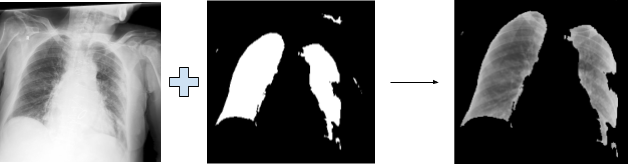
\includegraphics[width=8cm]{../doc/images/segmentation_training.png}
    \caption{Segmentation Training}
    \label{fig:segtrain}
\end{figure}

\subsubsection{FLANNEL}

In this section, we compare original FLANNEL base models and ensemble
performance with the patched FLANNEL. Because COVID-19 class is heavily
imbalanced compared to other categories, overall accuracy would not be the
appropriate measure for performance evaluation. It would not be able to show
performance increase in COVID-19 detection, So instead we use F1-score for
COVID-19 vs rest comparing the different models. As shown in Figure
\ref{fig:f1score}, we can see the ensemble approach in the original FLANNEL
clearly outperforms state-of-the-art base models in detecting COVID-19. We
however, don’t see the same performance gain in the patched FLANNEL approach
where ensemble performance is slightly worse than the original FLANNEL model. We
see a 1.17\% decrease in F1-score compared to original FLANNEL model. We do
notice significant improvement in all patched base models compared to the
original base models for COVID-19 detection.

\begin{figure*}[h]
    \centering
    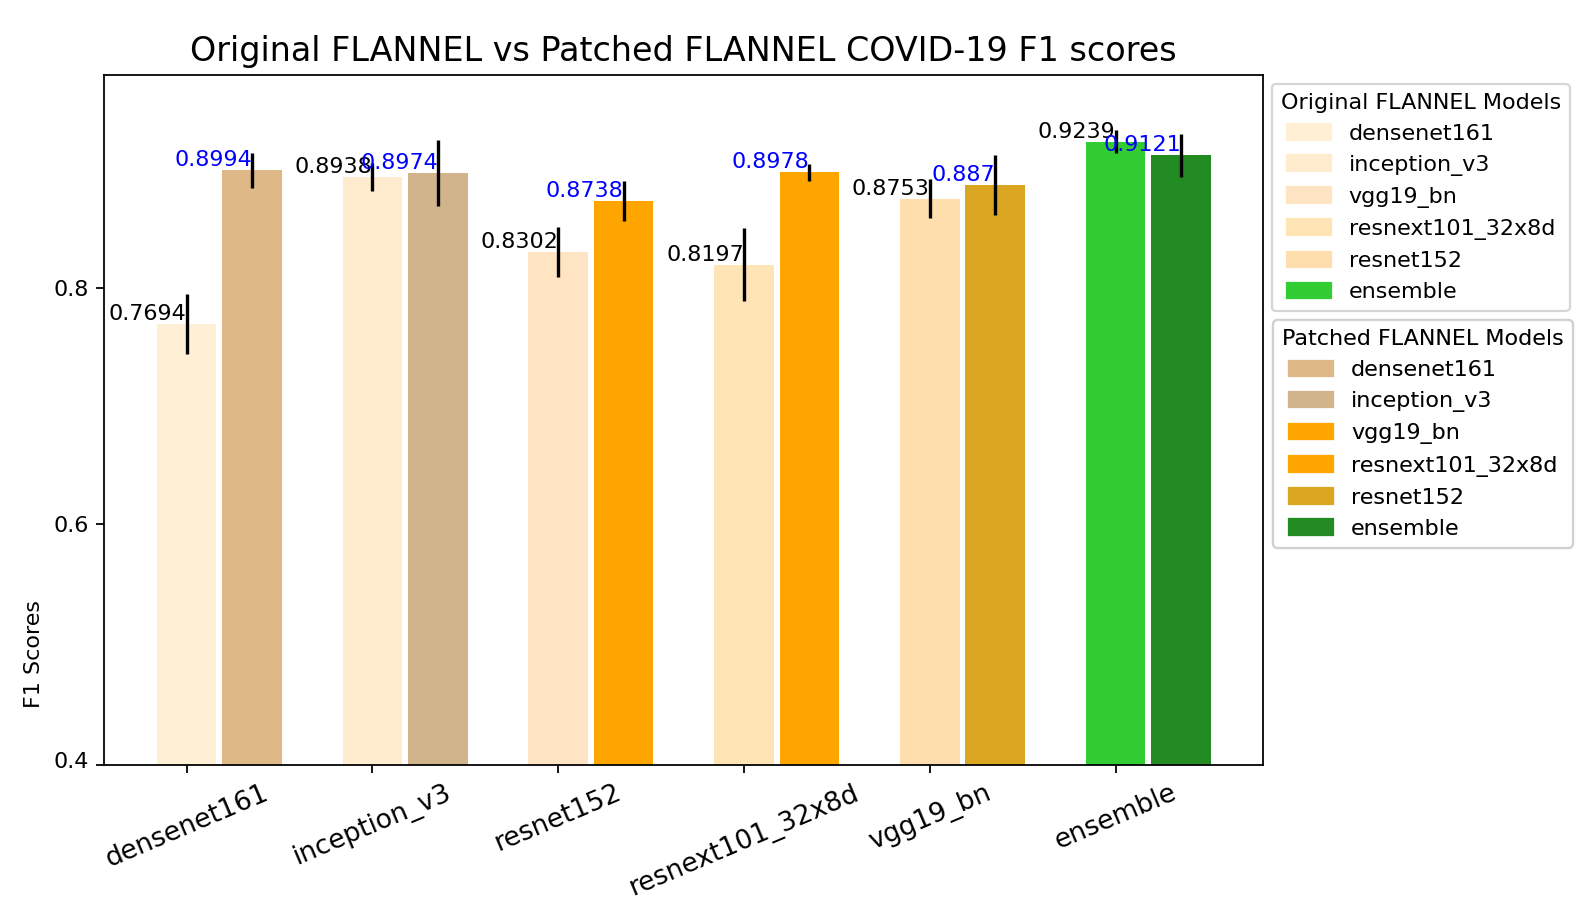
\includegraphics[width=0.8\textwidth]{../doc/images/original_vs_patched_flannel_f1.png}
    \caption{COVID-19 F1 score comparison}
    \label{fig:f1score}
\end{figure*}

\begin{figure*}[!htpb]
    \centering
    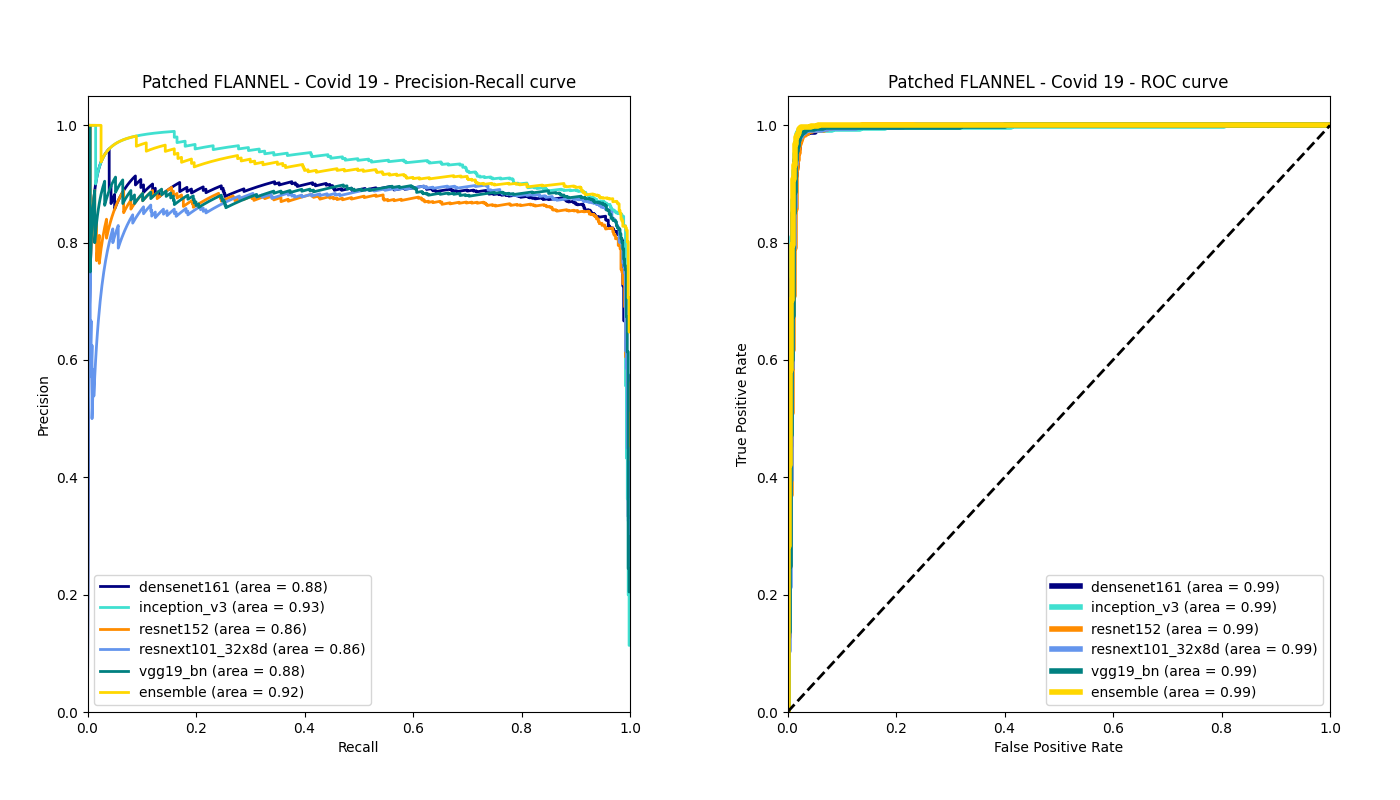
\includegraphics[width=0.8\textwidth]{../doc/images/patched_flannel_covid_19_plot_curve.png}
    \caption{Patched FLANNEL PR and ROC Curve}
    \label{fig:pf_roccurve}
\end{figure*}


In Table \ref{table:resultstats}, we show F1-score for each classification
and macro F1-score for all classes. In Table \ref{table:resultstats}, we can see
original FLANNEL performs better than base models and also performs better than
FLANNEL run with old dataset\cite{10.1093/jamia/ocaa280}. We see 13.11\% increase in performance of original
FLANNEL when run on new dataset. This can be attributed to now much better distribution
of COVID-19 images in current data. In patched based models, we see all base models
are performing better than original base models except for Pneumonia virus classification.
However, patched FLANNEL performs slightly poor in all four classification.
We see a decrease of 2.44\% in macro-F1 score for patched FLANNEL compared to
original FLANNEL.


We now compare the performance of the original FLANNEL ensemble with the patched
FLANNEL ensemble using micro-averaged precision and recall and see a slight
increase in overall performance compared to the original approach. This is
apparent in comparison of Precision-Recall curves in Figure \ref{fig:ec_prcurve}
and ROC (Receiver operating characteristic) curves in Figure
\ref{fig:ec_roccurve} of both ensemble method. As shown in Figure
\ref{fig:ec_prcurve} We see a 1.15\% increase in precision-recall AUC (Area
under curve) and 2.08\% increase in ROC AUC. As micro-average gives equal weight
to all predictions irrespective of classes. This shows patched ensemble model
performs slightly better in overall predictions.

\begin{figure}[h]
    \centering
    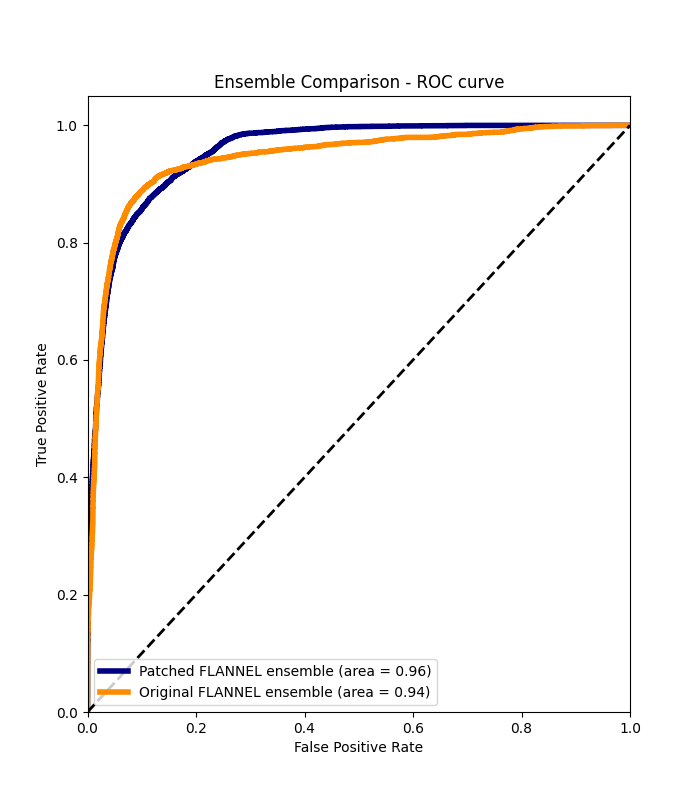
\includegraphics[width=7cm]{../doc/images/ensemble_comparison_roc_curve.png}
    \caption{EnsembLe Comparison ROC Curve}
    \label{fig:ec_roccurve}
\end{figure}

\begin{figure}[h]
    \centering
    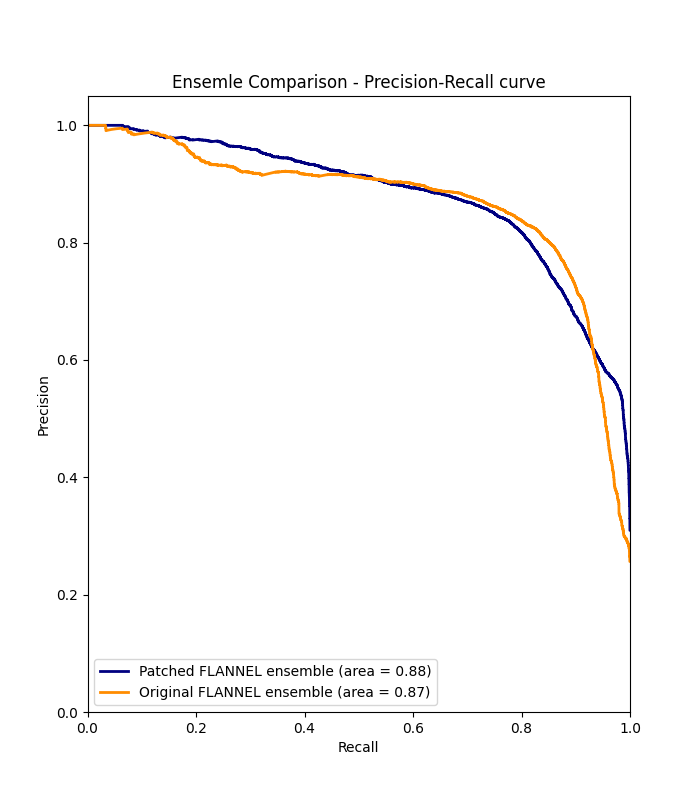
\includegraphics[width=7cm]{../doc/images/ensemble_comparison_precision_recall_curve.png}
    \caption{Ensemble Comparison PR Curve}
    \label{fig:ec_prcurve}
\end{figure}


We also compare the patched and original FLANNEL performance via confusion
matrix as shown in Figure \ref{fig:f_cf} and Figure \ref{fig:p_cf}. Due to
nature of random split between different runs, we see different numbers in both
confusion matrix. However it still provides enough information for us to compare.
We see patched and original FLANNEL performs similarly in detection of COVID-19 images
where it has higher precision and recall than other two types of Pneumonia. Both
models struggle with Pneumonia viral images classification and misclassifies
them as Pneumonia bacteria images.

\begin{figure}[h]
    \centering
    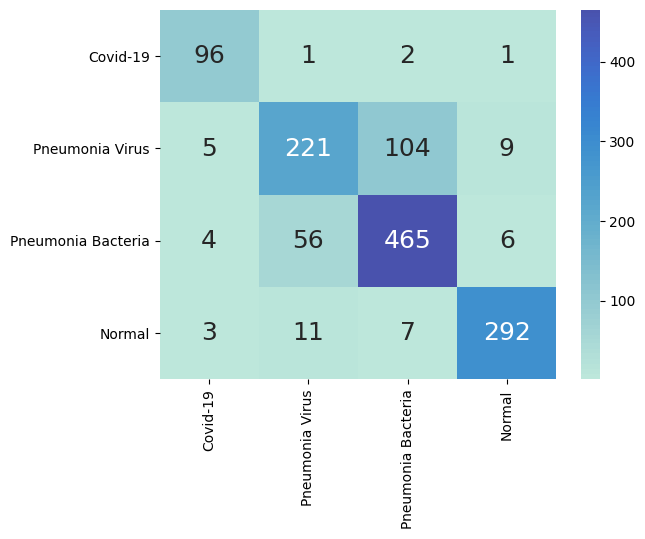
\includegraphics[width=7cm]{../doc/images/base_flannel_cf.png}
    \caption{Original FLANNEL Confusion Matrix}
    \label{fig:f_cf}
\end{figure}


\begin{figure}[h]
    \centering
    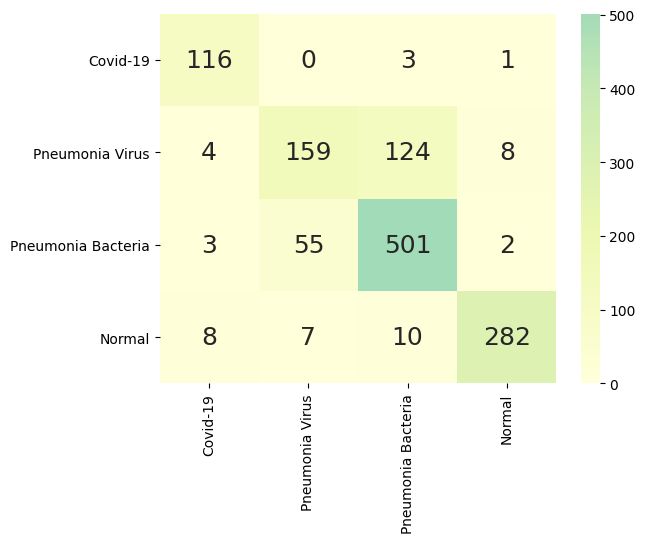
\includegraphics[width=7cm]{../doc/images/patched_flannel_cf.png}
    \caption{Patched FLANNEL Confusion Matrix}
    \label{fig:p_cf}
\end{figure}

We also present the ROC and Precision-Recall curve for COVID-19 classification
in Figure \ref{fig:pf_roccurve} to show diagnostic ability of patched FLANNEL.
We noted that ROC curve can be misleading for highly imbalanced classifications.
As we see using ROC curve AUC gives an impression of all models are performing
well as they have very few false positives. However when we look at PR curve, we
could see models performance differ and InceptionV3 and Ensemble model
performing better than others.


\section{Discussion}

We realized very early in the project that running FLANNEL model using five base
models and 200 epochs for five folds is going to take at least 3-4 days on a
high end GPU (Tesla V100 GPU or equivalent). We had to find a solution on both
cost and runtime in order to have results early. We tried multiple optimization
methods such as increasing the number of workers, mounting training images in
memory to bring the runtime down. We also used spot instances in parallel to
bring the cost down. We were able to faithfully reproduce original FLANNEL and
complete patched FLANNEL in a considerable short time with significantly low
cost. It took us 36 hours (144 compute hours) for original FLANNEL and 10 hours
(800 compute hours) for patched FLANNEL. The whole project costed us around
\$300.

Training the original FLANNEL model is already extremely slow as training single
model takes on average 2-3 hours. When using the original architecture for the
patch-based models, the training process was even slower due to two reasons. The
first is that the patch-base model data-loader was originally responsible for
applying the mask to the CXR image, this was addressed by transitioning the
responsibility to the segmentation task to immediately apply the mask to the
CXR. The second reason for the patch-based models being slow is that a
classification is run for each patch sequentially. This increases the complexity
from $N$ to $k\times N$ where $k$ is the number of patches. We were unable to
address this due to time constraints but we believe parallelizing the patch
predictions could lead to major improvements.

After training the patch-based models we were hoping to see substantial
improvements similar to Park et al. but we only noticed minor changes in
performance where some models slightly increased while others decreased. Two
models that had an increase in average precision performance were inceptionv3
and densenet161. While resnet152, resnext101 and vgg19\_bn had minor decreases
in average precision. Even though three of the base-models had decreased
performance, the patched ensemble still had a minor improvement over the base
ensemble in average precision by 1\%. We were originally hopeful to have more
significant increases in performance. Some of the reasons that could explain
this result is the segmentation that generated the masked CXR is inaccurate and
is masking important information surrounding the edges of the lungs. This
hypothesis will need to be verified by a medical expert. Another reason the
patch-based method was not as effective was that local patterns within the lung
areas of a CXR are less important than the global patterns detected within a
lung. This hypothesis can potentially be tested by increasing the patch size and
measuring performance again.

Some changes we made that could have decreased the patch-based model performance
are removing the weight assignment step from the patch classifier and limiting
the training to 100 epochs. The weight assignment step was removed because we
thought the probabilities of the classification output were already being passed
through an ensemble method where a neural network learns appropriate weights
based on class imbalance.


\section{Conclusion}
We had two major goals for this project. To faithfully reproduce FLANNEL on an
updated dataset with improved distribution of COVID-19 images and to apply
segmentation and patched classification to improve the COVID-19 detection
performance of FLANNEL model.

We ran the base models and FLANNEL ensemble on the new dataset using all five
folds and 200 epochs. With the improved distribution of COVID-19 data we see
FLANNEL outperforms the metrics as seen in the original FLANNEL paper by 13\%.
This large increase in performance highlights the importance of curating a rich
dataset.

Then we created the Segmentation model that produced masked CXR images that
displayed only the lung contours. These masked images were then used as a
dataset for patch-based versions of the FLANNEL model. The performance of the
patch-based models based on F1-Score had significant improvements when compared
with their original counterparts with the exception of the Pneumonia Viral
class. We then ran the ensemble on the outputs of the patch-based classifier
and did not note major improvement in classification performance. For COVID-19,
ensemble on patched classifiers performed slightly worse than Original FLANNEL
ensemble. However, for overall classification the average precision increased
by 1\% over the Original FLANNEL.

We trained patched base models for 100 epochs as done in the patch
classification paper and patched FLANNEL ensemble for 200 epochs.

We were partially able to achieve our goal of improving the original FLANNEL
architecture using patch-based models. Even though the performance was slightly
increased, we see both Original FLANNEL and Patched FLANNEL clearly outperforms
the other base models.

\section{Contribution}

All authors were actively involved in Patched FLANNEL development and
implementation. Major contributions from authors are:

\textbf{Maneesh:} AWS Setup, batch run of FLANNEL and patch-based models on
AWS, patch-based classification and ensemble model development, project
report, GitHub documentation

\textbf{Raman:} segmentation and patch-based classification development,
output graphs, presentation slide, project report, GitHub
documentation

\textbf{Satish:} FLANNEL checkpoints, output graphs and reports development,
GitHub documentation, presentation video

\textbf{Srikanth:} segmentation, patch-based classification development, project
report,GitHub documentation, presentation video

\section{Acknowledgement}
GitHub source code for both FLANNEL and Patch-Based classification
\cite{pmid32396075} paper are used as baseline for this improvement.
\begin{itemize}
    \item \href{https://github.com/qxiaobu/FLANNEL}{FLANNEL GitHub Repository}
    \item \href{https://github.com/jongcye/Deep-Learning-COVID-19-on-CXR-using-Limited-Training-Data-Sets}
          {Patch-Based classification}
\end{itemize}


\section{Appendix}
GitHub source code for the Patched FLANNEL
\url{https://github.com/mannbiher/DeepLearningForHealthCareProject}

\clearpage
%
% The following two commands are all you need in the initial runs of your .tex
% file to produce the bibliography for the citations in your paper.
\bibliographystyle{abbrv}
\bibliography{covid19}  % sigproc.bib is the name of the Bibliography in this

\end{document}
